% Markierungen: TODO
\documentclass{llncs}

\usepackage{etex}
\pagestyle{plain} % turn on page numbers
\usepackage[utf8]{inputenc}
\usepackage{microtype} % Better typesetting for PDFs -- is enabling this ok?
\usepackage{amsmath}
\usepackage{amssymb}
%\usepackage{eufrak} %The eufrak package is redundant if the amsfonts package is used
% \usepackage{mathpartir}
%\DeclareMathAlphabet{\mathpzc}{OT1}{pzc}{m}{it}
\usepackage[boxed]{algorithm}
\usepackage{enumerate}
\usepackage{listings}
\usepackage{graphicx}
\usepackage{tabularx}
\usepackage{booktabs}
\usepackage{color}
\usepackage[noend]{algpseudocode}
\usepackage{caption}
\usepackage[font=scriptsize]{subcaption}
\usepackage{hyperref}
\usepackage{float}
\usepackage{wrapfig}
\usepackage{multirow}
\usepackage{pgfplots}


\usepackage{packages/isabelle}
\usepackage{packages/isabelletags}
\usepackage{packages/isabellesym}
\usepackage{packages/comment}

% \isabellestyle{it}

\def\isachardoublequote{}%
\def\isachardoublequoteopen{}%
\def\isachardoublequoteclose{}%


\newcommand{\isainnerkeyword}[1]{{\tt #1}}
\newcommand{\isasymexistsA}{\isamath{\exists_{\textsc A}\,}}


\def\isadelimproof{}
\def\endisadelimproof{}
\def\isatagproof{}
\def\endisatagproof{}
\def\isafoldproof{}
\def\isadelimproof{}
\def\endisadelimproof{}

\input{lstisabelle}
\lstset{basicstyle=\footnotesize\ttfamily\slshape}
\lstset{captionpos=b}
\lstset{numberbychapter=false}

\newcommand{\isai}{\lstinline[language=isabelle,basicstyle=\normalsize\ttfamily\slshape]}




\input{macros}

% Include snippets
\newcommand{\DefineSnippet}[2]{%
   \expandafter\newcommand\csname snippet--#1\endcsname{%
     \begin{quote}
     \begin{isabelle}\footnotesize
     #2
     \end{isabelle}
     \end{quote}}}
\newcommand{\Snippet}[1]{\ifcsname snippet--#1\endcsname\csname snippet--#1\endcsname\else\PackageError{}{No snippet '#1' defined.}{}\fi}
\DefineSnippet{ford_fulkerson_algo}{
\isacommand{definition}\isamarkupfalse%
\ {\isachardoublequoteopen}ford{\isacharunderscore}fulkerson{\isacharunderscore}method\ {\isasymequiv}\ \isainnerkeyword{do}\ {\isacharbraceleft}\isanewline
\ \ \isainnerkeyword{let}\ f\ {\isacharequal}\ {\isacharparenleft}{\isasymlambda}{\isacharparenleft}u{\isacharcomma}v{\isacharparenright}{\isachardot}\ {\isadigit{0}}{\isacharparenright}{\isacharsemicolon}\isanewline
\isanewline
\ \ {\isacharparenleft}f{\isacharcomma}brk{\isacharparenright}\ {\isasymleftarrow}\ \isainnerkeyword{while}\isanewline
\ \ \ \ {\isacharparenleft}{\isasymlambda}{\isacharparenleft}f{\isacharcomma}brk{\isacharparenright}{\isachardot}\ {\isasymnot}brk{\isacharparenright}\ \isanewline
\ \ \ \ {\isacharparenleft}{\isasymlambda}{\isacharparenleft}f{\isacharcomma}brk{\isacharparenright}{\isachardot}\ \isainnerkeyword{do}\ {\isacharbraceleft}\isanewline
\ \ \ \ \ \ p\ {\isasymleftarrow}\ \isainnerkeyword{selectp}\ p{\isachardot}\ is{\isacharunderscore}augmenting{\isacharunderscore}path\ f\ p{\isacharsemicolon}\isanewline
\ \ \ \ \ \ \isainnerkeyword{case}\ p\ of\ \isanewline
\ \ \ \ \ \ \ \ None\ {\isasymRightarrow}\ \isainnerkeyword{return}\ {\isacharparenleft}f{\isacharcomma}True{\isacharparenright}\isanewline
\ \ \ \ \ \ {\isacharbar}\ Some\ p\ {\isasymRightarrow}\ \isainnerkeyword{return}\ {\isacharparenleft}augment\ c\ f\ p{\isacharcomma}\ False{\isacharparenright}\isanewline
\ \ \ \ {\isacharbraceright}{\isacharparenright}\isanewline
\ \ \ \ {\isacharparenleft}f{\isacharcomma}False{\isacharparenright}{\isacharsemicolon}\isanewline
\ \ \isainnerkeyword{return}\ f\ \isanewline
{\isacharbraceright}{\isachardoublequoteclose}%
}%EndSnippet
\DefineSnippet{ford_fulkerson_correct}{
\isacommand{theorem}\isamarkupfalse%
\ {\isacharparenleft}\isakeyword{in}\ Network{\isacharparenright}\ {\isachardoublequoteopen}ford{\isacharunderscore}fulkerson{\isacharunderscore}method\ {\isasymle}\ {\isacharparenleft}\isainnerkeyword{spec}\ f{\isachardot}\ isMaxFlow\ f{\isacharparenright}{\isachardoublequoteclose}%
}%EndSnippet
\DefineSnippet{edmonds_karp_correct}{
\isacommand{theorem}\isamarkupfalse%
\isanewline
\ \ \isakeyword{fixes}\ el\ \isakeyword{defines}\ {\isachardoublequoteopen}c{\isasymequiv}ln{\isacharunderscore}{\isasymalpha}\ el{\isachardoublequoteclose}\isanewline
\ \ \isakeyword{shows}\ {\isachardoublequoteopen}{\isacharless}emp{\isachargreater}\ edmonds{\isacharunderscore}karp\ el\ s\ t\ {\isacharless}{\isasymlambda}\isanewline
\ \ \ \ \ \ None\ {\isasymRightarrow}\ {\isasymup}{\isacharparenleft}{\isasymnot}ln{\isacharunderscore}invar\ el\ {\isasymor}\ {\isasymnot}Network\ c\ s\ t{\isacharparenright}\isanewline
\ \ \ \ {\isacharbar}\ Some\ {\isacharparenleft}N{\isacharcomma}cf{\isacharparenright}\ {\isasymRightarrow}\ \isanewline
\ \ \ \ \ \ {\isasymup}{\isacharparenleft}ln{\isacharunderscore}invar\ el\ {\isasymand}\ Network\ c\ s\ t\ {\isasymand}\ Graph{\isachardot}V\ c\ {\isasymsubseteq}\ {\isacharbraceleft}{\isadigit{0}}{\isachardot}{\isachardot}{\isacharless}N{\isacharbraceright}{\isacharparenright}\isanewline
\ \ \ \ {\isacharasterisk}\ {\isacharparenleft}{\isasymexistsA}f{\isachardot}\ is{\isacharunderscore}rflow\ c\ N\ f\ cf\ {\isacharasterisk}\ {\isasymup}{\isacharparenleft}Network{\isachardot}isMaxFlow\ c\ s\ t\ f{\isacharparenright}{\isacharparenright}{\isachargreater}\isactrlsub t{\isachardoublequoteclose}%
}%EndSnippet
\DefineSnippet{augment_flow_presv_cap}{
\isacommand{lemma}\isamarkupfalse%
\ augment{\isacharunderscore}flow{\isacharunderscore}presv{\isacharunderscore}cap{\isacharcolon}\ \isanewline
\ \ \isakeyword{shows}\ {\isachardoublequoteopen}{\isadigit{0}}\ {\isasymle}\ {\isacharparenleft}f{\isasymup}f{\isacharprime}{\isacharparenright}{\isacharparenleft}u{\isacharcomma}v{\isacharparenright}\ {\isasymand}\ {\isacharparenleft}f{\isasymup}f{\isacharprime}{\isacharparenright}{\isacharparenleft}u{\isacharcomma}v{\isacharparenright}\ {\isasymle}\ c{\isacharparenleft}u{\isacharcomma}v{\isacharparenright}{\isachardoublequoteclose}\isanewline
%
\isadelimproof
%
\endisadelimproof
%
\isatagproof
\isacommand{proof}\isamarkupfalse%
\ {\isacharparenleft}cases\ {\isachardoublequoteopen}{\isacharparenleft}u{\isacharcomma}v{\isacharparenright}{\isasymin}E{\isachardoublequoteclose}{\isacharsemicolon}\ rule\ conjI{\isacharparenright}\ \isanewline
\ \ \isacommand{assume}\isamarkupfalse%
\ {\isacharbrackleft}simp{\isacharbrackright}{\isacharcolon}\ {\isachardoublequoteopen}{\isacharparenleft}u{\isacharcomma}v{\isacharparenright}{\isasymin}E{\isachardoublequoteclose}\isanewline
\ \ \isacommand{hence}\isamarkupfalse%
\ {\isachardoublequoteopen}f{\isacharparenleft}u{\isacharcomma}v{\isacharparenright}\ {\isacharequal}\ cf{\isacharparenleft}v{\isacharcomma}u{\isacharparenright}{\isachardoublequoteclose}\ \isanewline
\ \ \ \ \isacommand{using}\isamarkupfalse%
\ no{\isacharunderscore}parallel{\isacharunderscore}edge\ \isacommand{by}\isamarkupfalse%
\ {\isacharparenleft}auto\ simp{\isacharcolon}\ residualGraph{\isacharunderscore}def{\isacharparenright}\isanewline
\ \ \isacommand{also}\isamarkupfalse%
\ \isacommand{have}\isamarkupfalse%
\ {\isachardoublequoteopen}cf{\isacharparenleft}v{\isacharcomma}u{\isacharparenright}\ {\isasymge}\ f{\isacharprime}{\isacharparenleft}v{\isacharcomma}u{\isacharparenright}{\isachardoublequoteclose}\ \isacommand{using}\isamarkupfalse%
\ f{\isacharprime}{\isachardot}capacity{\isacharunderscore}const\ \isacommand{by}\isamarkupfalse%
\ auto\isanewline
\ \ \isacommand{finally}\isamarkupfalse%
\ \isacommand{have}\isamarkupfalse%
\ {\isachardoublequoteopen}f{\isacharprime}{\isacharparenleft}v{\isacharcomma}u{\isacharparenright}\ {\isasymle}\ f{\isacharparenleft}u{\isacharcomma}v{\isacharparenright}{\isachardoublequoteclose}\ \isacommand{{\isachardot}}\isamarkupfalse%
\isanewline
%
\isanewline
%
\ \
\isacommand{have}\isamarkupfalse%
\ {\isachardoublequoteopen}{\isacharparenleft}f{\isasymup}f{\isacharprime}{\isacharparenright}{\isacharparenleft}u{\isacharcomma}v{\isacharparenright}\ {\isacharequal}\ f{\isacharparenleft}u{\isacharcomma}v{\isacharparenright}\ {\isacharplus}\ f{\isacharprime}{\isacharparenleft}u{\isacharcomma}v{\isacharparenright}\ {\isacharminus}\ f{\isacharprime}{\isacharparenleft}v{\isacharcomma}u{\isacharparenright}{\isachardoublequoteclose}\isanewline
\ \ \ \ \isacommand{by}\isamarkupfalse%
\ {\isacharparenleft}auto\ simp{\isacharcolon}\ augment{\isacharunderscore}def{\isacharparenright}\isanewline
\ \ \isacommand{also}\isamarkupfalse%
\ \isacommand{have}\isamarkupfalse%
\ {\isachardoublequoteopen}{\isasymdots}\ {\isasymge}\ f{\isacharparenleft}u{\isacharcomma}v{\isacharparenright}\ {\isacharplus}\ f{\isacharprime}{\isacharparenleft}u{\isacharcomma}v{\isacharparenright}\ {\isacharminus}\ f{\isacharparenleft}u{\isacharcomma}v{\isacharparenright}{\isachardoublequoteclose}\isanewline
\ \ \ \ \isacommand{using}\isamarkupfalse%
\ {\isacartoucheopen}f{\isacharprime}{\isacharparenleft}v{\isacharcomma}u{\isacharparenright}\ {\isasymle}\ f{\isacharparenleft}u{\isacharcomma}v{\isacharparenright}{\isacartoucheclose}\ \isacommand{by}\isamarkupfalse%
\ auto\isanewline
\ \ \isacommand{also}\isamarkupfalse%
\ \isacommand{have}\isamarkupfalse%
\ {\isachardoublequoteopen}{\isasymdots}\ {\isacharequal}\ f{\isacharprime}{\isacharparenleft}u{\isacharcomma}v{\isacharparenright}{\isachardoublequoteclose}\ \isacommand{by}\isamarkupfalse%
\ auto\isanewline
\ \ \isacommand{also}\isamarkupfalse%
\ \isacommand{have}\isamarkupfalse%
\ {\isachardoublequoteopen}{\isasymdots}\ {\isasymge}\ {\isadigit{0}}{\isachardoublequoteclose}\ \isacommand{using}\isamarkupfalse%
\ f{\isacharprime}{\isachardot}capacity{\isacharunderscore}const\ \isacommand{by}\isamarkupfalse%
\ auto\isanewline
\ \ \isacommand{finally}\isamarkupfalse%
\ \isacommand{show}\isamarkupfalse%
\ {\isachardoublequoteopen}{\isacharparenleft}f{\isasymup}f{\isacharprime}{\isacharparenright}{\isacharparenleft}u{\isacharcomma}v{\isacharparenright}\ {\isasymge}\ {\isadigit{0}}{\isachardoublequoteclose}\ \isacommand{{\isachardot}}\isamarkupfalse%
\isanewline
\ \ \ \ \ \ \isanewline
\ \ \isacommand{have}\isamarkupfalse%
\ {\isachardoublequoteopen}{\isacharparenleft}f{\isasymup}f{\isacharprime}{\isacharparenright}{\isacharparenleft}u{\isacharcomma}v{\isacharparenright}\ {\isacharequal}\ f{\isacharparenleft}u{\isacharcomma}v{\isacharparenright}\ {\isacharplus}\ f{\isacharprime}{\isacharparenleft}u{\isacharcomma}v{\isacharparenright}\ {\isacharminus}\ f{\isacharprime}{\isacharparenleft}v{\isacharcomma}u{\isacharparenright}{\isachardoublequoteclose}\ \isanewline
\ \ \ \ \isacommand{by}\isamarkupfalse%
\ {\isacharparenleft}auto\ simp{\isacharcolon}\ augment{\isacharunderscore}def{\isacharparenright}\isanewline
\ \ \isacommand{also}\isamarkupfalse%
\ \isacommand{have}\isamarkupfalse%
\ {\isachardoublequoteopen}{\isasymdots}\ {\isasymle}\ f{\isacharparenleft}u{\isacharcomma}v{\isacharparenright}\ {\isacharplus}\ f{\isacharprime}{\isacharparenleft}u{\isacharcomma}v{\isacharparenright}{\isachardoublequoteclose}\ \isacommand{using}\isamarkupfalse%
\ f{\isacharprime}{\isachardot}capacity{\isacharunderscore}const\ \isacommand{by}\isamarkupfalse%
\ auto\isanewline
\ \ \isacommand{also}\isamarkupfalse%
\ \isacommand{have}\isamarkupfalse%
\ {\isachardoublequoteopen}{\isasymdots}\ {\isasymle}\ f{\isacharparenleft}u{\isacharcomma}v{\isacharparenright}\ {\isacharplus}\ cf{\isacharparenleft}u{\isacharcomma}v{\isacharparenright}{\isachardoublequoteclose}\ \isacommand{using}\isamarkupfalse%
\ f{\isacharprime}{\isachardot}capacity{\isacharunderscore}const\ \isacommand{by}\isamarkupfalse%
\ auto\isanewline
\ \ \isacommand{also}\isamarkupfalse%
\ \isacommand{have}\isamarkupfalse%
\ {\isachardoublequoteopen}{\isasymdots}\ {\isacharequal}\ f{\isacharparenleft}u{\isacharcomma}v{\isacharparenright}\ {\isacharplus}\ c{\isacharparenleft}u{\isacharcomma}v{\isacharparenright}\ {\isacharminus}\ f{\isacharparenleft}u{\isacharcomma}v{\isacharparenright}{\isachardoublequoteclose}\ \isanewline
\ \ \ \ \isacommand{by}\isamarkupfalse%
\ {\isacharparenleft}auto\ simp{\isacharcolon}\ residualGraph{\isacharunderscore}def{\isacharparenright}\isanewline
\ \ \isacommand{also}\isamarkupfalse%
\ \isacommand{have}\isamarkupfalse%
\ {\isachardoublequoteopen}{\isasymdots}\ {\isacharequal}\ c{\isacharparenleft}u{\isacharcomma}v{\isacharparenright}{\isachardoublequoteclose}\ \isacommand{by}\isamarkupfalse%
\ auto\isanewline
\ \ \isacommand{finally}\isamarkupfalse%
\ \isacommand{show}\isamarkupfalse%
\ {\isachardoublequoteopen}{\isacharparenleft}f{\isasymup}f{\isacharprime}{\isacharparenright}{\isacharparenleft}u{\isacharcomma}\ v{\isacharparenright}\ {\isasymle}\ c{\isacharparenleft}u{\isacharcomma}\ v{\isacharparenright}{\isachardoublequoteclose}\ \isacommand{{\isachardot}}\isamarkupfalse%
\isanewline
\isacommand{qed}\isamarkupfalse%
\ {\isacharparenleft}auto\ simp{\isacharcolon}\ augment{\isacharunderscore}def\ cap{\isacharunderscore}positive{\isacharparenright}%
\endisatagproof
{\isafoldproof}%
%
\isadelimproof
%
\endisadelimproof
%
}%EndSnippet



% \overfullrule=8pt

\begin{document}

\title{Formalizing the Edmonds-Karp Algorithm}
% \subtitle{}

\author{Peter Lammich, S.~Reza Sefidgar}

\institute{Technische Universit\"at M\"unchen, \email{\{lammich,sefidgar\}@in.tum.de}}

\maketitle
\begin{abstract}
We present a formalization of the Ford-Fulkerson method for computing the maximum flow in a network.
Our formal proof closely follows a standard textbook proof, and is accessible even without being
an expert in Isabelle/HOL --- the interactive theorem prover used for the formalization.
We then use stepwise refinement to obtain the Edmonds-Karp algorithm, and formally prove a bound on its complexity.
Further refinement yields a verified implementation, whose execution time compares well to an unverified reference implementation in Java.

%We present a formalization of the Ford-Fulkerson method for computing the maximum flow in a network. 
%The formal proofs are done in Isabelle/HOL. They closely follow a standard textbook proof and are relatively easy 
%to read, even without being an Isabelle expert.

%We then use stepwise refinement to obtain the Edmonds-Karp algorithm and prove its upper complexity bound of $O(|V||E|^2)$.
%Further refinement yields a verified implementation, which is almost as fast as an unverified  
%reference implementation in Java. 

% 
% and a verified imperative implementation of it. Our implementation is roughly 2.5 times slower than an unverified  
% reference implementation in Java. 
% 
% Finally, we prove the upper complexity bound of $O(|V||E|^2)$ for the Edmonds-Karp algorithm.
\end{abstract}

\section{Introduction}
Computing the maximum flow of a network is an important problem in graph theory.
Many other problems, like maximum-bipartite-matching, edge-disjoint-paths, circulation-demand, as well as various scheduling and resource allocating problems can be reduced to it.
The Ford-Fulkerson method~\cite{FF56} describes a class of algorithms to solve the maximum flow problem. An important instance is the Edmonds-Karp algorithm~\cite{EK72},
which was one of the first algorithms to solve the maximum flow problem in polynomial time for the general case of networks with real-valued capacities.

In this paper, we present a formal verification of the Edmonds-Karp algorithm and its polynomial complexity bound.
The formalization is conducted in the Isabelle/HOL proof assistant~\cite{NPW02}. 
Stepwise refinement techniques~\cite{Wirth71,Back78,BaWr98} allow us to elegantly structure our verification into an abstract proof of the Ford-Fulkerson method,
its instantiation to the Edmonds-Karp algorithm, and finally an efficient implementation. The abstract parts of our verification closely follow the textbook presentation of Cormen et al.~\cite{CLRS09}. Using the Isar~\cite{Wenzel99} proof language, we were able to produce proofs that are accessible even to non-Isabelle experts.

While there exists another formalization of the Ford-Fulkerson method in Mizar~\cite{Lee05}\footnote{Section~\ref{sec:related_work} provides a detailed discussion}, we are, to the best of our knowledge, the first that verify a polynomial maximum flow algorithm, prove the polynomial complexity bound, or provide a verified executable implementation. Moreover, this paper is a case study on elegantly formalizing algorithms.

The rest of this paper is structured as follows: In Section~\ref{sec:background} we give a short informal introduction to the Ford-Fulkerson method.
In Section~\ref{sec:abs-formalization}, we report on our formalization of the abstract method. 
Section~\ref{sec:refinement} gives a brief overview of the Isabelle Refinement Framework~\cite{LaTu12,La12}, which supports stepwise refinement based algorithm development in Isabelle/HOL. In Section~\ref{sec:edka}, we report on our instantiation of the Ford-Fulkerson method to the Edmonds-Karp algorithm and the proof of its complexity.
Section~\ref{sec:executable} reports on the further refinement steps required to yield an efficient implementation. Section~\ref{sec:benchmark} reports on 
benchmarking our implementation against a reference implementation of the Edmonds-Karp algorithm from Sedgewick et al.~\cite{SeWa11}. 
Finally, Section~\ref{sec:concl} gives a conclusion and discusses related and future work. The source code of our formalization is available at \url{http://www21.in.tum.de/~lammich/edmonds_karp/}.


% Despite its importance, no formalization of the Ford-Fulkerson algorithm has been developed in modern proof assistants. The only similar work that the authors are aware of is formalization of the Ford-Fulkerson algorithm in Mizar~\cite{Lee05}. This formalization defines and proves correctness of the algorithm at the level of graph manipulations without providing concrete implementation of the algorithm. Providing such an implementation is specially important, as it could provide the basis for many verfied programs with practical importance.

\section{The Ford-Fulkerson Method}\label{sec:background}
% \begin{comment}
%   GOAL: 
%     1) Remind the reader of FoFu. The educated reader should have the feeling:
%       Yes, now I recall FoFu, and understand (again) what it does.
%       
%     2) Set the field for further, more detailed descriptions in next section.
%   
% 
%   Short description of Network: Finite graph over nodes V, 
%     edge (u,v) annotated with capacity c(u,v).
%     Assuming distinct nodes s and t. 
%     Note on additional assumptions: 
%         No parallel edges, s only outgoing, t only incoming, all nodes on path from s to t. 
%         Can transform any Network to match these assumptions, preserving the flow cite{???}.
%         
%   s-t Flow: Annotation of edges with values, such that: 
%     1) Values smaller than capacities.
%     2) Kirchhoff law: sum of incoming flows = sum of outgoing flows, for all nodes except s t
%   
%   Value of flow: Incoming flow - outgoing flow of s
%   
%   Max-Flow problem. 
%     Rpt. why important?
%   
%   Cuts, intuition of min-cut >= max-flow
%   
%   Theorem: Min-Cut = Max-Flow
%   Proven via augmenting flow in residual graph. 
%     Present 1,2,3 of min-cut max-flow equivalences
%   
%   This yields an algorithm to compute max-flows, if we can compute flows in residual graph.
%     --> Simple way: Augmenting flow via augmenting path. ==> FoFu-scheme. 
%       Termination? In General: Only for integer capacities.
%       Edmonds-Karp: Shortest augmenting path. Always terminates! Complexity: O(|E||V|) outer loop iterations, BFS requires O|E|.
%   \end{comment}

In this section, we give a short introduction to the Ford-Fulkerson method, closely following the presentation by Cormen et al.~\cite{CLRS09}.

% TODO: Possible alternative presentation
%   First define a relaxed network, without the constraints. Define the flow there. Then add network constraints.
% 

A (flow) network is a directed graph over a finite set of vertices $V$ and edges $E$, where each edge $(u,v)\in E$ is labeled by a positive real-valued capacity $c(u,v)>0$.
Moreover, there are two distinct vertices $s,t\in V$, which are called \emph{source} and \emph{sink}. 

A \emph{flow} $f$ on a network is a labeling of the edges with real values satisfying the following constraints: 1) \emph{Capacity constraint}: the flow on each edge is a non-negative value smaller or equal to the edge's capacity; 2) \emph{Conservation constraint}: For all vertices except $s$ and $t$, the sum of flows over all incoming edges is equal to the sum of flows over all outgoing edges. 
The value of a flow $f$ is denoted by $|f|$, and defined to be the sum over the outgoing flows of $s$ minus the sum over the incoming flows of $s$.
Given a network $G$, the maximum flow problem is to find a flow with a maximum value among all flows of the network. 

To simplify reasoning about the maximum flow problem, we assume that our network satisfies some additional constraints: 1) the source only has outgoing edges while the sink only has incoming edges; 2) if the network contains an edge $(u, v)$ then there is no \emph{parallel edge} $(v, u)$ in the reverse direction\footnote{With $u=v$, this also implies that there are no self loops.}; and 3) every vertex of the network must be on a path from $s$ to $t$. Note that any network can be transformed to a network with the aforementioned properties and the same maximum flow~\cite{CLRS09}.


An important result is the relation between flows and cuts in a network. A \emph{cut} is a partitioning of the vertices into two sets, such that one set contains 
the source and the other set contains the sink. The capacity of a cut is the sum of the capacities of all edges going from the source's side to the sink's side of the cut.
It is easy to see that the value of any flow cannot exceed the capacity of any cut, as all flow from the source must ultimately reach the sink, and thus go through the edges of the cut. The Ford-Fulkerson theorem tightens this bound and states that the value of the maximum flow is equal to the capacity of the minimum cut.

The Ford-Fulkerson method is a corollary of this theorem. It is based on a greedy approach: Starting from a zero flow, the value of the flow is iteratively increased until a maximum flow is reached. In order to increase the overall flow value, it may be necessary to redirect some flow, \ie to decrease the flow passed through specific edges. For this purpose the Ford-Fulkerson method defines the residual graph, which has edges in the same and opposite direction as the network edges.
% , which has edges both in parallel and reverse to the edges of the network. 
Each edge is labeled by the amount of flow that can be effectively passed along this edge, by either increasing or decreasing the flow on a network edge.
Formally, the residual graph $G_f$ of a flow $f$ is the graph induced by the 
edges with positive labels according to the following labeling function $c_f$:
\[ c_f (u, v) = 
  \begin{cases}
  c (u, v) - f(u, v) \hfill & \text{ if $(u, v) \in E$} \\
  f (v, u) \hfill & \text{ if $(v, u) \in E$} \\  
  0 \hfill & \text{ otherwise} \\
  \end{cases} 
\]

In each iteration, the Ford-Fulkerson method tries to find an \emph{augmenting path}, \ie a simple path from $s$ to $t$ in the residual graph.
It then pushes as much flow as possible along this path to increase the value of the current flow. 
Formally, for an augmenting path $p$, one first defines the \emph{residual capacity} $c_p$ as the minimum value over all edges of $p$:
\[c_f(p) = \min \{c_f(u, v): \text{$(u, v)$ is on  $p$}\}\]
An augmenting path then yields a residual flow $f_p$, which is the flow that can be passed along this path:
\[ f_p (u, v) = 
  \begin{cases}
  c_f(p) \hfill & \text{ if $(u, v)$ is on $p$} \\  
  0 \hfill & \text{ otherwise} \\
  \end{cases} 
\]
\newcommand{\augment}{{\mathbin\uparrow}}%
Finally, to actually push the flow induced by an augmenting path, we define the \emph{augment} function $f\augment f'$, which augments a flow $f$ in the network 
by any \emph{augmenting flow} $f'$, \ie any flow in the residual graph:
\[ (f \augment f') (u, v) = 
  \begin{cases}
  f (u, v) + f'(u, v) - f'(v, u) \hfill & \text{ if $(u, v) \in E$} \\  
  0 \hfill & \text{ otherwise} \\
  \end{cases} 
\]
Note that, for any edge in the network, the augmenting flow in the same direction is added to the flow, while the augmenting flow in the opposite direction is subtracted. 
This matches the intuition of passing flow in the indicated direction, by either increasing or decreasing the flow of an edge in the network.

The correctness of the Ford-Fulkerson algorithm follows from the Ford-Fulkerson theorem, which is usually stated as the following three statements being equivalent:
\begin{enumerate}
\item $f$ is a maximum flow in a network $G$.
\item there is no augmenting path in the residual graph $G_f$.
\item there is a cut $C$ in $G$ such that the capacity of $C$ is equal to the value of $f$.
\end{enumerate}

The Ford-Fulkerson method does not specify how to find an augmenting path in the residual graph. There are several possible implementations with different execution times. The general method is only guaranteed to terminate for networks with rational capacities, while it may infinitely converge against non-maximal flows in the case of irrational edge capacities~\cite{FF56,Zwick95}. When always choosing a \emph{shortest} augmenting path, the number of iterations is bound by $O(VE)$, even for the general case of real-valued capacities. Note that we write $V$ and $E$ instead of $|V|$ and $|E|$ for the number of nodes and edges if the intended meaning is clear from the context.
A shortest path can be found by breadth first search (BFS) in time $O(E)$, yielding the Edmonds-Karp algorithm~\cite{EK72} with an overall running time of $O(VE^2)$. 


\section{Formalizing the Ford-Fulkerson Method}\label{sec:abs-formalization}
%  GOAL: Present highlights of our formalization, persuade the reader that we have done something substantial.
%    Reader should think: Yeah, they did cool stuff!
%
%  [???* Thematize definition of flows: On Graphs vs. on Networks. You find both in the literature. 
%      We decides for [...]. This is better suited, as is gives nice and elegant proofs, even formally, bla bla bla]
%    
%  Proof of MinCut-MaxFlow: Follows the textbook proof.
%    Uses Isar to even look like a textbook proof, being comprehensible even without running
%      Isabelle/HOL.
%      
%    For example, \isai{augment_flow_presv_cap}.
%      Present formal proof text. Perhaps oppose it to textbook proof?.
%    
%  Abstract Algo looks like pseudocode presented in texbooks.
%    Oppose our algo to textbook pseudocode.
%    

%A formal proof contains many technical details that are not presented in an informal proof. While dealing with the technical details in a proof causes distraction, leaving out such details makes it hard to follow the proofs.  . So, readers may use this informal proof as a guide to better understand the relevant thoughts in our formal proof. Moreover using the proof language Isar, we made the formal proof readable even for readers that are not familiar with Isabelle.

In this section, we provide a brief overview of our formalization of the Ford-Fulkerson method. 
In order to develop theory in the context of a fixed graph or network, we use Isabelle's concept of \emph{locales}~\cite{Ballarin:2006:MKM}, which allows
us to define named contexts that fix some parameters and assumptions.
For example, the graph theory is developed in the locale \isai{Graph}, which 
fixes the edge labeling function \isai{c}, and defines the set of edges and nodes based on $c$:
\begin{lstlisting}
  locale Graph = fixes c :: "edge => capacity" begin
    definition "E == {(u, v). c (u, v) ~= 0}"
    definition "V == {u. \<exists>v. (u, v) \<in> E \<or> (v, u) \<in> E}"
    [...]
\end{lstlisting}
Moreover, we define basic concepts like (simple, shortest) paths, and provide lemmas to reason about them.

Networks are based on graphs, and add the source and sink nodes, as well as the network assumptions:
\begin{lstlisting}
  locale Network = Graph + fixes s t :: node
    assumes no_incoming_s: "\<forall>u. (u, s) \<notin> E"
    [...]
\end{lstlisting}
Most theorems presented in this paper are in the context of the \isai{Network} locale.

\subsection{Presentation of Proofs}
% (DONE: not sure about repeating citation of Cormen: I would definitely repeat the citation!) 
Informal proofs focus on the relevant thoughts by leaving out technical details and obvious steps. 
In contrast, a formal proof has to precisely specify each step as the application of some inference rules. 
Although modern proof assistants provide high-level tactics to summarize some of these steps, formal proofs tend to be significantly more 
verbose than informal proofs. Moreover, formal proofs are conducted in the tactic language of the proof assistant, which is often some dialect of ML. 
Thus, many formal proofs are essentially programs that instruct the proof assistant how to conduct the proof. They tend to be inaccessible without a deep knowledge of the used proof assistant, in many cases requiring to replay the proof in the proof assistant in order to understand the idea behind it.

For the Isabelle/HOL proof assistant, the Isar proof language~\cite{Wenzel99} allows to write formal proofs that resemble standard mathematical textbook proofs, and are accessible, to a certain extent, even for those not familiar with Isabelle/HOL. 
We use Isar to present our proof of the Ford-Fulkerson method such that it resembles the informal proof described by Cormen et al.~\cite{CLRS09}.

As an example, consider the proof that for a flow $f$ and a residual flow $f'$, the augmented flow $f\augment f'$ is again a valid flow. In particular, one has to show 
that the augmented flow satisfies the capacity constraint. Cormen et al.~give the following proof, which we display literally here, only replacing the references to 
``Equation~26.4'' by ``definition of $\augment$'':

For the capacity constraint, first observe that if $(u, v) \in E$, then $c_f(v, u) = f(u, v)$. Therefore, we have $f'(v,u) \leq c_f(v, u) = f(u, v)$, and hence
	\begin{align*}
	(f \uparrow f') (u, v) &= f(u, v) + f'(u, v) - f'(v, u)  && \text{(definition of $\augment$)} \\
	& \geq f(u, v) + f'(u, v) - f(v, u) && \text{(because $f'(v,u) \leq f(u, v)$)} \\
	& = f'(u, v) \\
	& \geq 0.
	\end{align*}
In addition,
	\begin{align*}
	(f \uparrow f') (u, v) &= f(u, v) + f'(u, v) - f'(v, u)  && \text{(definition of $\augment$)} \\
	& \leq f(u, v) + f'(u, v) && \text{(because flows are nonnegative)} \\
	& \leq f(u, v) + c_f(u, v) &&  \text{(capacity constraint)} \\
	& = f(u, v) + c(u, v) - f(u, v) && \text{(definition of $c_f$)} \\
	& = c (u, v).
	\end{align*}
% 
In the following we present the corresponding formal proof in Isar:
\Snippet{augment_flow_presv_cap}
The structure of the Isar proof is exactly the same as that of the textbook proof, except that we had to also consider the case $(u,v)\notin E$, which is not mentioned in the informal proof at all, and easily discharged in our formal proof by the \isai{auto}-tactic after the \isai{qed}. We also use exactly the same justifications as the original proof, except that we had to use the fact that there are no parallel edges to show $c_f(v,u)=f(u,v)$, which is not mentioned in the original proof.

\subsection{Presentation of Algorithms}
In textbooks, it is common to present algorithms in pseudocode, which captures the essential ideas, but leaves open implementation details. As a formal equivalent to pseudocode, we use the monadic programming language provided by the Isabelle Refinement Framework~\cite{LaTu12,La12}. For example, we define the Ford-Fulkerson method as follows:
\Snippet{ford_fulkerson_algo}

% DONE: Introduce obtain-syntax, and unfold find-augmenting-path spec! Or even while-exists loop as combinator?
The code looks quite similar to pseudocode that one would expect in a textbook, but actually is a rigorous formal specification of the algorithm, using nondeterminism to leave open the implementation details (\cf Section~\ref{sec:refinement}). Note that we had to use the available combinators of the Isabelle Refinement Framework, which made the code slightly more verbose than we would have liked. We leave it to future work to define a set of combinators and appropriate syntax that allows for more concise presentation of pseudocode.

% The only caveat is that our framework currently does not support breaking of loops, such that we had to use an explicit flag instead. 

Finally, using the Ford-Fulkerson theorem and the verification condition generator of the Isabelle Refinement Framework, it is straightforward to prove (partial) correctness of
the Ford-Fulkerson method, which is stated in Isabelle/HOL by the following theorem:
\Snippet{ford_fulkerson_correct}

\section{Refinement in Isabelle/HOL}\label{sec:refinement}
After having stated and proved correct an algorithm on the abstract level, the next step is to provide an (efficient) implementation. 
In our case, we first specialize the Ford-Fulkerson method to use shortest augmenting paths, then implement the search for shortest augmenting paths by BFS, and finally use efficient data structures to represent the abstract objects modified by the algorithm. 

A natural way to achieve this formally is \emph{stepwise refinement}~\cite{Wirth71}, and in particular \emph{refinement calculus}~\cite{Back78,BaWr98}, which allows us to systematically transform an abstract algorithm into a more concrete one, preserving its correctness.

In Isabelle/HOL, stepwise refinement is supported by the Isabelle Refinement Framework~\cite{LaTu12,La12}. 
It features a refinement calculus for programs phrased in a nondeterminism monad. 
The monad's type is a set of possible results plus an additional value that indicates a failure:
\begin{lstlisting}
  datatype \<alpha> nres = res \<alpha> set | fail
\end{lstlisting}
The operation \isai{return x} of the monad describes the single result \isai{x}, and the 
operation \isai{bind m f} nondeterministically picks a result from \isai{m} and executes \isai{f} on it. 
The bind operation fails iff either \isai{m = fail}, or \isai{f} may fail for a result in \isai{m}, 

We define the \emph{refinement ordering} on \isai{\<alpha> nres} by lifting the subset ordering with \isai{fail} being the greatest element.
Intuitively, \isai{m <= m'} means that \isai{m} is a refinement of \isai{m'}, \ie all possible results of \isai{m} are 
also possible results of \isai{m'}. 
Note that the refinement ordering is a complete lattice, and bind is monotonic. Thus, we can define recursion using a fixed-point construction~\cite{Kr10}.
Moreover, we can use the standard Isabelle/HOL constructs for if, let and case distinctions, yielding a fully fledged programming 
language, shallowly embedded into Isabelle/HOL's logic. For simpler usability, we define standard loop constructs (while, foreach), 
a syntax for postcondition specifications, and use a Haskell-like do-notation:
\begin{lstlisting}
  spec P == spec x. P x == res {x. P x}
  do {x <- m; f x} == bind m f
  do {m; m'} == bind m (%_. m')
\end{lstlisting}

Correctness of a program \isai{m} with precondition \isai{P} and postcondition \isai{Q} is expressed as \isai{P ==> m <= spec r. Q r} (or, eta-contracted, just \isai{spec Q}), which
means that, if \isai{P} holds, \isai{m} does not fail and all possible results of \isai{m} satisfy \isai{Q}. Note that we provide different recursion constructs
for partial and total correctness: A nonterminating total correct recursion yields \isai{fail}, which satisfies no specification, even if joined 
with results from other possible runs. On the other hand, a nonterminating partial correct recursion yields \isai|res {}|, which refines any specification 
and disappears when joined with other results.

The Isabelle Refinement Framework also supports data refinement. The representation of results can be changed according to a \emph{refinement relation}, 
which relates concrete with abstract results: Given a relation \isai{R}, \isai{\<Down>R m} is the set of concrete results that are related to an 
abstract result in \isai{m} by \isai{R}. If \isai{m = fail}, then also \isai{\<Down>R m = fail}.

In a typical program development, one first comes up with an initial version \isai{m_0} of
the algorithm and its specification \isai{P,Q}, and shows \isai{P ==> m_0 <= spec Q}. Then, one iteratively provides refined versions \isai{m$_i$} of the algorithm,
proving \isai{m$_i$ <= \<Down>R$_i$ m$_{i-1}$}. Using transitivity and composability of data refinement, one 
gets \isai{P ==> m$_i$ <= \<Down>R$_i$...R$_1$ spec Q}, showing the correctness of the refined algorithm.
If no data refinement is performed, \isai{R$_i$} is set to the identity relation, in which case \isai{\<Down>R$_i$} becomes the identity function.

Various tools, including a verification condition generator, assist the user in conducting the refinement proofs by breaking 
them down to statements that do not contain monad constructs any more. In many cases, these verification conditions reflect the core idea of the proof precisely.

Monotonicity of the standard combinators also allows for modular refinement: Replacing a part of a program by a refined version
results in a program that refines the original program. This gives us a natural formal model for statements like ``we implement shortest path finding by BFS'', or ``we use arrays to represent the edge labeling''. 

% 
% 
% Purpose: Separation of concerns.
% 
% Short intro on Refinement Framework:
% 
% Programs phrased as error-set monad. With order structure. 
% Refinement: Less possible results (refinement ordering). Error is greatest element (refined by everything).
% 
% Building chains of refinement, at the end there should be a deterministic algorithm (yielding exactly one result), which is
% contained (by transitivity) in the specification.
% 
% Standard combinators (bind, recursion, if, etc) are monotonic wrt. refinement ordering, which allows for modularity:
% Replacing part of a program by a refined version, yields a refined program. 
% 
% Data refinement: Changing the representation of data. Relation between concrete and abstract representation. 
% $\Uparrow m$ is biggest concrete program that refines $m$ wrt.\ relation $R$. 
% 
% The Isabelle Refinement Framework provides the nres-monad, and tools to reason about program refinement, 
% the most important one being a VCG.




\section{The Edmonds-Karp Algorithm}\label{sec:edka}
  Specializing the Ford-Fulkerson method to the Edmonds-Karp algorithm is straightforward, as finding a shortest augmenting path is a refinement of finding any augmenting path.
  
  Considerably more effort is required to show that the resulting algorithm terminates within $O(VE)$ iterations. 
  The idea of the proof is as follows: Edges in the opposite direction to an edge on a shortest path cannot lie 
  on a shortest path itself.
%   that are reverse to edges on a shortest path cannot lie 
%   on a shortest path itself.
  On every augmentation, at least one edge of the residual graph that lies on a shortest augmenting path is flipped. Thus, either the length of the shortest path increases,
  or the number of edges that lie on some shortest path decreases. As the length of a shortest path is at most $V$, there are no more than $O(VE)$ iterations.
  % TODO: Add more explanation here, like: DIstinguish two cases: 1) ... 2) The distance s-t in cf is still the same, but then ...
  
  Note that Cormen et al.~present the same idea a bit differently: They define an edge of the residual graph being \emph{critical} if it lies on a shortest path such that it will be flipped by augmentation. Then, they establish an upper bound of how often an edge can get critical during the algorithm. Our presentation is more suited for a formal proof, as we can directly construct a measure function from it, \ie a function from flows to natural numbers, which decreases on every iteration and is bounded by $O(VE)$. 
  
  Formalizing the above intuitive argument was more tricky than it seemed on first glance:
  While it is easy to prove that, in a \emph{fixed graph}, an edge and its opposite cannot both lie on shortest paths, generalizing the argument
  to a graph transformation which may add multiple flipped edges and removes at least one original edge requires some generalization of the statement.
  Note that a straightforward induction on the length of the augmenting path or on the number of flipped edges fails, as, after flipping the first 
  edge, the path no longer exists.
  
%   We decided to generalize the statement as follows. Assume we have an original graph $cf$ with a shortest augmenting path $p$, and a transformed graph $cf'$ that has been created from
%   $cf$ by adding some flipped edges from $p$ and removing some edges from $p$.
%   Then, we consider an edge $(u,v) \in p$, a path $p_1$ from $s$ to $v$ in the original graph, and a path $p_2$ from $u$ to $t$ in the transformed graph.
%   
%   By induction on the number of reversed edges in $p_2$, we 
%   show that $|p_1|+|p_2| > |p|$. In the induction step, we use the proof idea for the single flipped edge $(v,u)$, and,
%   if $p_2$ contains more flipped edges, we split $p_2$ at the first flipped edge. Then, the initial segment of $p_2$ contains no flipped edges,
%   and thus also is a path in the original graph, and we can apply the induction hypothesis.
%   
%   Proving that augmentation with a shortest augmenting path actually only adds flipped edges, and removes at least one original edge, required some more work,
%   but was straightforward and yielded no surprises.
%   
%   Finally, we phrase the complexity argument as a measure function $m = l*2|E| + n$, where $l$ is the length of the shortest augmenting path,
%   and $n$ is the number of edges that lie on any shortest path. We show that $m$ is decreased by the loop body.
%   Adding a special case for loop termination (there are no augmenting paths), and observing that $m$ is bounded by $2|V||E|$, yields 
%   the desired upper bound on loop iterations. Refinement of the algorithm to add an explicit loop counter, and asserting the upper bound, is then straightforward.
  
  Having defined the measure function and shown that it decreases on augmentation, it is straightforward to refine the partial correct while loop to a total correct one. Moreover, to make explicit the bound on the number of loop iterations, we instrument the loop to count its iterations, and assert the upper bound after the loop.


    
\section{Refinement to Executable Code}\label{sec:executable}
  In the previous section, we have presented our abstract formalization of the Edmonds-Karp algorithm,
  leaving open how to obtain a shortest augmenting path and how to implement the algorithm. 
  In this section, we outline the further refinement steps that were necessary to obtain an efficient implementation.

  \subsection{Using Breadth First Search}
  A standard way to find a shortest path in a graph is breadth first search (BFS). Luckily, we had already formalized a BFS algorithm as an example for the 
  Isabelle Refinement Framework. Unfortunately, this algorithm only computed the minimum distance between two nodes, without returning an actual path. For this project, we extended the formalization accordingly, and added an efficient imperative implementation, using the same stepwise refinement techniques as for the main algorithm. Note that the resulting BFS algorithm is independent, and can be reused for finding shortest paths in other applications. 
  
  Implementing shortest path finding by BFS in Edmonds-Karp algorithm yields a specification that algorithmically describes all major operations, but still leaves open the data structures used for implementation.
  
%   
%   We briefly report on our adapted formalization here, which is displayed in Figure~\ref{TODO: Snippet}: 
%   TODO: Reference to figure (line numbers?)
%   The abstract algorithm keeps track of a set $C$ of current nodes, a set $N$ of new nodes, and a partial map $P$ from already visited nodes to predecessor nodes.
%   Initially, only the start node is in $C$ and $N$ is empty. In each iteration of the loop, a node $u\in C$ is picked, and its successors $v$ that have not yet been 
%   visited are added to $N$, and $P~v$ is set to $u$. If $C$ becomes empty, $C$ and $N$ are swapped. If the target node is encountered, the algorithm immediately terminates.
%   Note that this implementation is a generalized version of the usual queue implementation of BFS: While a queue enforces a complete order on the encountered nodes, our 
%   implementation only enforces an ordering between nodes on the current level and nodes on the next level. 
% 
%   For the actual algorithm, we wrap this algorithm by a procedure to handle the special case where source and target nodes are the same, and to extract a shortest path 
%   from $P$ upon termination. Moreover, we implement the abstract specification of adding the successor nodes of a node by a loop.
%   
%   Finally, we prove the following theorem: %TODO: Not actually true, the impls are oly done in bfs2!
% %     theorem
% %       assumes "src∈V" 
% %       shows "bfs src dst ≤ (spec p. 
% %         case p of None ⇒ ¬conn src dst | Some p ⇒ shortestPath src p dst)"
%   
%   Obviously, the BFS algorithm refines the specification for obtaining a shortest path.
%   Using this to refine the Edmonds-Karp formalization yields a program that algorithmically specifies all major operations.
     
  \subsection{Manipulating Residual Graphs Directly}\label{sec:impl_res_graph}
  Next, we observe that the algorithm is phrased in terms of a flow, which is updated until it is maximal. 
  In each iteration, the augmenting path is searched on the residual graph induced by the current flow.
  Obviously, computing the complete residual graph in each iteration is a bad idea. 
  One solution to this problem is to compute the edges of the residual graph on the fly from the network and the current flow.
  Although this solution seems to be common, it has the disadvantage that for each edge of the residual graph, two (or even three) 
  edges of the network and the flow have to be accessed. As edges of the residual graph are accessed in the inner loop, during 
  the BFS, these operations are time critical.
  
  After our profiling indicated a hot spot on accessing the capacity matrices of the network and the flow, we switched to 
  an algorithm that operates on a representation of the residual graph directly. This resulted in a speed-up of roughly a factor of two.
  As the residual graph uniquely determines the flow (and vice versa), it is straightforward to phrase the
  operations directly on the residual graph. Performing a data refinement of the flow \wrt the refinement 
  relation $\{(c_f,f) \mid \text{$f$ is a flow}\}$ then yields the desired algorithm.
      
  \subsection{Implementing Augmentation}    
  In our abstract formalization, which matches the presentation in Section~\ref{sec:background}, we have formulated augmentation by first defining 
  the residual capacity $c_p$ of the augmenting path. Using $c_p$, we have defined the residual flow $f_p$, which was finally added to the current flow.
  In the refinement to operate on residual graphs, we have refined this to augment the residual graph.
  For the implementation, we compute the residual capacity in a first iteration over the augmenting path, and modify the residual graph 
  in a second iteration. Proving this implementation correct is straightforward by induction on the augmenting path.
      
  \subsection{Computing Successors}
  In order to find an augmenting path, the BFS algorithm has to compute the successors of a node in the residual graph. 
  Although this can be implemented on the edge labeling function by iterating over all nodes, this implementation tends to be inefficient for sparse graphs,
  where we would have to iterate over many possible successor nodes just to find that there is no edge. 
  
  A common optimization is to pre-compute an \emph{adjacency map} from nodes to adjacent nodes in the network. 
  As an edge in the residual graph is either in the same or opposite direction of 
  a network edge, it is enough to iterate over the adjacent nodes in the network, and check whether they are actual successors in the residual graph.
  It is straightforward to show that this implementation actually returns the successor nodes in the residual graph.

  \subsection{Using Efficient Data Structures}\label{sec:impl_data_structures}
  In a final step, we have to choose efficient data structures for the algorithm. 

  %   The objects that the algorithm works with are
%   capacities, nodes, edges, the graph of the input network, residual graphs, the adjacency map, paths, and the resulting maximum flow. 
  
  We implement capacities as (arbitrary precision) integer numbers\footnote{Up to this point, the formalization models capacities as \emph{linearly ordered integral domains}, which subsume reals, rationals, and integers. Thus, we could chose any executable number representation here.}. Note that an implementation as fixed precision numbers would also be possible,
  but requires additional checks on the network to ensure that no overflows can happen. 
  % TODO: Can we trick the Java reference implementation on integer overflow?
  
  We implement nodes as natural numbers less than an upper bound $N$, and residual graphs are implemented by their capacity matrices, which, in turn,
  are realized as arrays of size $N\times N$ with row-major indexing, such that the successors of a node are close together in memory.
  The adjacency map of the network is implemented as an array of lists of nodes. 
  An augmenting path is represented by a list of edges, \ie a list of pairs of nodes. 
  
  
%   For the BFS algorithm, we implement the sets $C$ and $N$ by lists, and the predecessor map $P$ as an array of \isai{node option}. 
%   The successors of a node are represented as a list with no duplicate elements. The resulting path, which is extracted from $P$ upon termination of
%   the BFS, is represented as a list of edges. 
  
  
  The input network of the algorithm is represented as a function from network edges to capacities, which is tabulated into an array
  to obtain the initial residual graph. This gives us some flexibility in using the algorithm, as any capacity matrix representation can be converted into a 
  function easily, without losing efficiency for read-access. 
  Similarly, our implementation expects an adjacency map as additional parameter, which is then tabulated into an array. This is convenient in our context, where a preprocessing step computes the adjacency map anyway.
      
  The output flow of the algorithm is represented as the residual graph. The user can decide how to compute the maximum flow from it. For example,
  in order to compute the maximum flow value, only the outgoing edges of the source node have to be computed, which is typically less 
  expensive than computing the complete flow matrix. The correctness theorem of the algorithm abstractly states how to obtain the maximum flow from the output.

  Note that there is still some optimization potential left in the choice of our data structures: 
  For example, the BFS algorithm computes a predecessor map $P$. It then iterates over $P$ to extract the shortest path as a list of edges.
  A subsequent iteration over this list computes the residual capacity, and a final iteration performs the augmentation. 
  This calls for a deforestation optimization to get rid of the intermediate list, and iterate only two times over the predecessor map directly.
%   A first time to compute the bottleneck, and a second time to do the augmentation. 
  Fortunately, iteration over the shortest path seems not to significantly contribute to the runtime of our implementation, such that 
  we leave this optimization for future work.

  Note that we performed the last refinement step using our Sepref tool~\cite{La15,La16}, which provides tool support for refinement from the
  purely functional programs of the Isabelle Refinement Framework into imperative programs expressed in Imperative/HOL~\cite{BKHEM08}.
  The formalization of this refinement step consists of setting up the mappings between the abstract and concrete data structures,
  and then using Sepref to synthesize the Imperative/HOL programs and their refinement proofs.
  Finally, Imperative/HOL comes with a setup for the Isabelle code generator~\cite{Haft09,HaNi10} to generate imperative programs in OCaml, SML, Scala, and Haskell.

  \subsection{Network Checker}
  Additionally, we implemented an algorithm that takes as input a list of edges, a source node, and a target node.
  It converts these to a capacity matrix and an adjacency map, and checks whether the resulting graph satisfies our network assumptions.
  We proved that this algorithm returns the correct capacity matrix and adjacency map iff the input describes a valid network,
  and returns a failure value otherwise.
    
  Combining the implementation of the Edmonds-Karp algorithm with the network checker yields our final implementation,
  for which we can export code, and have proved the following theorem: 
  
  \vspace{\abovedisplayskip}{\raggedright\begin{minipage}{\textwidth}
  \Snippet{edmonds_karp_correct}
  \end{minipage}}\vspace{\belowdisplayskip}
  
  \noindent Note that this theorem is stated as a Hoare triple, using separation logic~\cite{Rey02,LaMe12} assertions. There are no preconditions on the input.
  If the algorithm returns \isai{None}, then the edge list was malformed or described a graph that does not satisfy the network assumptions.
  Here, \isai{ln_invar} describes well-formed edge lists, \ie edge lists that have no duplicate edges and only edges with positive capacity,
  and \isai{ln_\<alpha>} describes the mapping from (well-formed) edge lists to capacity matrices (note that we set \isai{c == ln_\<alpha> el}).
  If the algorithm returns some number \isai{N} and residual graph \isai{cf}, then the input was a well-formed edge list that describes a valid network with at most \isai{N} nodes.
  Moreover, the returned residual graph describes a flow \isai{f} in the network, which is maximal. 
  As the case distinction is exhaustive, this theorem states the correctness of the algorithm. 
  Note that Isabelle/HOL does not have a notion of execution, thus total correctness of the generated code cannot be expressed. However, the program is phrased in a heap-exception monad, thus introducing some (coarse grained) notion of
  computation. On this level, termination can be ensured, and, indeed, the above theorem implies that all the recursions stated by recursion 
  combinators in the monad must terminate. However, it does not guarantee that we have not injected spurious code equations like $f~x = f~x$, 
  which is provable by reflexivity, but causes the generated program to diverge.

\section{Benchmarking}\label{sec:benchmark}
  We have compared the running time of our algorithm in SML against an unverified reference implementation in Java, taken from Sedgewick and Wayne's book on algorithms~\cite{SeWa11}. We have used MLton 20100608~\cite{MLton} and OpenJDK Java 1.7.0\_95, running on a standard laptop machine with a 2.8GHz i7 quadcore processor and 16GiB of RAM.
  
  We have done the comparison on randomly generated sparse and dense networks, the sparse networks having a \emph{density} (${} = \frac{E}{V(V - 1)}$) of $0.02$, and the dense networks having a density of $0.25$. Note that the maximum density for networks that satisfy our assumptions is $0.5$, as we allow no parallel edges.
  For sparse networks, we varied the number of nodes between $1000$ and $5500$, for dense networks between $1000$ and $1450$.
  The results are shown in Figure~\ref{fig:benchmark}, in a double-logarithmic scale.
 
  \begin{figure}[!h]
  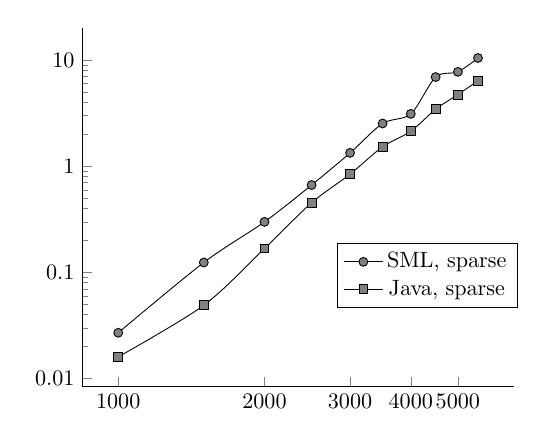
\begin{tikzpicture}[thick,scale=.8, every node/.style={scale=1}] %change the scales if you like to reduce the size
    \begin{axis}[
      %title={Benchmark of the Edmonds-Karp algorithm},
        axis x line*= bottom,
        axis y line*= left,
        xmode = log,
        ymode = log,
%         xlabel = Number of vertices in the network,
%         ylabel = Execution time in seconds, 
        xtick = {0,1000,...,5000},
        ytick = {0.01,0.1,1,10},
        xticklabels = {$1000$, $2000$, $3000$, $4000$, $5000$},
        yticklabels = {$0.01$,$0.1$,$1$,$10$}, 
        smooth,
        cycle list name = black white,
        legend style = { 
          at={(0.59,0.4)}, 
            anchor=north west,
            draw=black, 
            fill= white,
            align=left
        }
    ]
    
    %start data for plotting
      \addplot table {
        1000 .027   
        1500 .124  
        2000 .299  
        2500 .665  
        3000 1.335 
        3500 2.526 
        4000 3.111 
        4500 6.917 
        5000 7.743 
        5500 10.452    
      }; \addlegendentry{SML, sparse};

      \addplot table {
        1000 .016   
        1500 .049   
        2000 .168  
        2500 .453  
        3000 .842  
        3500 1.524 
        4000 2.136 
        4500 3.438 
        5000 4.734 
        5500 6.369     
      }; \addlegendentry{Java, sparse};
    %end data for plotting
    \end{axis}
  \end{tikzpicture}
%
  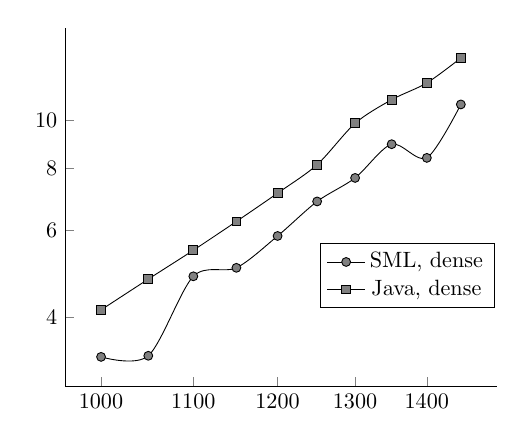
\begin{tikzpicture}[thick,scale=.8, every node/.style={scale=1}] %change the scales if you like to reduce the size
    \begin{axis}[
      %title={Benchmark of the Edmonds-Karp algorithm},
        axis x line*= bottom,
        axis y line*= left,
        xmode = log,
        ymode = log,
%         xlabel = Number of vertices in the network,
%         ylabel = Execution time in seconds, 
        xtick = {0,1000,1100,...,1400},
        ytick = {2,4,...,10},
        xticklabels = {$1000$, $1100$, $1200$, $1300$, $1400$}, 
        yticklabels = {$2$, $4$,$6$,$8$,$10$}, 
        smooth,
        cycle list name = black white,
        legend style = { 
          at={(0.59,0.4)}, 
            anchor=north west,
            draw=black, 
            fill= white,
            align=left
        }
    ]
    
    %start data for plotting
      \addplot table {
        1000 3.328 
        1050 3.345 
        1100 4.841 
        1150 5.036 
        1200 5.840 
        1250 6.858 
        1300 7.651 
        1350 8.950 
        1400 8.398 
        1450 10.769     
      }; \addlegendentry{SML, dense};

      \addplot table {
        1000 4.141 
        1050 4.778 
        1100 5.465 
        1150 6.248 
        1200 7.128 
        1250 8.137 
        1300 9.864 
        1350 11.008
        1400 11.902
        1450 13.365     
      }; \addlegendentry{Java, dense};
    %end data for plotting
    \end{axis}
  \end{tikzpicture}
  
  
  
%   \centering    
%   \begin{tikzpicture}[thick,scale=1, every node/.style={scale=1}] %change the scales if you like to reduce the size
%     \begin{axis}[
%       %title={Benchmark of the Edmonds-Karp algorithm},
%         axis x line*= bottom,
%         axis y line*= left,
%         xmode = log,
%         ymode = log,
%         xlabel = Number of vertices in the network,
%         ylabel = Execution time in milliseconds, %in milliseconds, modify the scale for lables
%         xtick = {0,1000,...,5000},
% %         ytick = data,
%         xticklabels = {$1000$, $2000$, $3000$, $4000$, $5000$}, %corresponds to the first column in {SML, Sparse}
% %         yticklabels = {$0.2$, $1.4$, $4.9$, $9.2$, $23.6$}, %corresponds to the second column in {SML, Sparse}
%         smooth,
%         cycle list name = black white,
%         legend style = { 
%           at={(0.59,0.4)}, 
%             anchor=north west,
%             draw=black, 
%             fill= white,
%             align=left
%         }
%     ]
%     
%     %start data for plotting
%       \addplot table {
%         1000 27   
%         1500 124  
%         2000 299  
%         2500 665  
%         3000 1335 
%         3500 2526 
%         4000 3111 
%         4500 6917 
%         5000 7743 
%         5500 10452    
%       }; \addlegendentry{SML, sparse};
% 
%       \addplot table {
%         1000 16   
%         1500 49   
%         2000 168  
%         2500 453  
%         3000 842  
%         3500 1524 
%         4000 2136 
%         4500 3438 
%         5000 4734 
%         5500 6369     
%       }; \addlegendentry{Java, sparse};
% 
%       \addplot table {
%         1000 3328 
%         1050 3345 
%         1100 4841 
%         1150 5036 
%         1200 5840 
%         1250 6858 
%         1300 7651 
%         1350 8950 
%         1400 8398 
%         1450 10769     
%       }; \addlegendentry{SML, dense};
% 
%       \addplot table {
%         1000 4141 
%         1050 4778 
%         1100 5465 
%         1150 6248 
%         1200 7128 
%         1250 8137 
%         1300 9864 
%         1350 11008
%         1400 11902
%         1450 13365     
%       }; \addlegendentry{Java, dense};
%     %end data for plotting
%     \end{axis}
%   \end{tikzpicture}
  
%   \center{\footnotesize The x-axis shows the number of nodes, the y axis the execution time in seconds.}
  \caption{Benchmark of different implementations. The x-axis shows the number of nodes, the y axis the execution time in seconds.}\label{fig:benchmark}
  \end{figure}

  We observe that, for sparse graphs, the Java implementation is roughly faster by a factor of $1.6$, while for dense graphs, our implementation is faster by a factor of $1.2$. Note that the Java implementation operates on flows, while our implementation 
  operates on residual graphs (\cf Section~\ref{sec:impl_res_graph}). Moreover, the Java implementation does not store the augmenting 
  path in an intermediate list, but uses the predecessor map computed by the BFS directly (\cf Section~\ref{sec:impl_data_structures}).
  Finally note that a carefully optimized C++ implementation of the algorithm is only slightly faster than the Java implementation for sparse graphs,
  but roughly one order of magnitude faster for dense graphs. We leave it to future work to investigate this issue, and conclude that we were able to produce
  a reasonably fast verified implementation.
  
%   , without doing any low-level optimizations, but using the code as generated by the Isabelle/HOL code generator.
  
% 
%   What implementations did we compare: Authors? Where do implementations come from? 
%   [We must convince the reader that we did not intentionally chose bad implementations to compare us against!]
% 
%   Comparsion of algorithms (Modified data structure: Flow vs Flow-like vs ResGraph)
%     Computing successors in BFS: Filter by visited set first.
%       -> Technically more challenging, when computing on flow: 1 access first vs 2 accesses first. On resGraph: No advantage in memory accesses (However, plain array access vs. matrix access)
%     Computing bottleneck during BFS. Saves one iteration over the path, at the cost of one extra memory access per discovered node.
%     For our benchmarks, we observed that the BFS discovers considerably more nodes than the length of the ultimately returned path, 
%     and the overall code was faster with the extra iteration for bottleneck computation.
    
    

\section{Conclusion}\label{sec:concl}
  We have presented a verification of the Edmonds-Karp algorithm, using a stepwise refinement approach.
  Starting with a proof of the Ford-Fulkerson theorem, we have verified the generic Ford-Fulkerson method, 
  specialized it to the Edmonds-Karp algorithm, and proved the upper bound $O(VE)$ for the number of outer loop iterations.
  We then conducted several refinement steps to derive an efficiently executable implementation of the algorithm, 
  including a verified breadth first search algorithm to obtain shortest augmenting paths. 
  Finally, we added a verified algorithm to check whether the input is a valid network, and generated executable code in SML.
  The runtime of our verified implementation compares well to that of an unverified reference implementation in Java.
  
  Our formalization has combined several techniques to achieve an elegant and accessible formalization: 
  Using the Isar proof language~\cite{Wenzel99}, we were able to provide a completely rigorous but 
  still accessible proof of the Ford-Fulkerson theorem. The Isabelle Refinement Framework~\cite{LaTu12,La12} and the Sepref tool~\cite{La15,La16}
  allowed us to present the Ford-Fulkerson method on a level 
  of abstraction that closely resembles pseudocode presentations found in textbooks, and then formally link this presentation to an efficient
  implementation. Moreover, modularity of refinement allowed us to develop the breadth first search algorithm independently, and later link it to the 
  main algorithm. The BFS algorithm can be reused as building block for other algorithms. The data structures are re-usable, too: although we had to implement the array representation of (capacity) matrices for this project, it will be added to the growing library of verified imperative data structures 
  supported by the Sepref tool, such that it can be re-used for future formalizations.
  
  During this project, we have learned some lessons on verified algorithm development: 
  \begin{itemize}
  \item It is important to keep the levels of abstraction strictly separated.
    For example, when implementing the capacity function with arrays, one needs to show that it is only applied to valid nodes.
    However, proving that, e.g., augmenting paths only contain valid nodes is hard at this low level. 
    Instead, one can protect the application of the capacity function by an assertion--- already on a high abstraction level where it can be easily discharged. 
    On refinement, this assertion is passed down, and ultimately available for the implementation.
    Optimally, one wraps the function together with an assertion of its precondition into a new constant, which is then refined independently.
  \item Profiling has helped a lot in identifying candidates for optimization. For example, based on profiling data, we decided to delay a 
    possible deforestation optimization on augmenting paths, and to first refine the algorithm to operate on residual graphs directly.
  \item ``Efficiency bugs'' are as easy to introduce as for unverified software. For example, out of convenience, we implemented the successor list computation by
    \emph{filter}. Profiling then indicated a hot-spot on this function. As the order of successors does not matter, we invested a bit more work to make the computation tail 
    recursive and gained a significant speed-up. Moreover, we realized only lately that we had accidentally implemented and verified
    matrices with column major ordering, which have a poor cache locality for our algorithm. Changing the order resulted in another significant speed-up.
  \end{itemize}
  
  We conclude with some statistics:
  The formalization consists of roughly 8000 lines of proof text, where the graph theory up to the Ford-Fulkerson algorithm requires 3000 lines.
  The abstract Edmonds-Karp algorithm and its complexity analysis contribute 800 lines, and its implementation (including BFS) another 1700 lines.
  The remaining lines are contributed by the network checker and some auxiliary theories. The development of the theories required roughly 3 man month, a significant amount of this time going into a first, purely functional version of the implementation, which was later dropped in favor of the faster imperative version.
  
  
  \subsection{Related Work}\label{sec:related_work}
  We are only aware of one other formalization of the Ford-Fulkerson method conducted in Mizar~\cite{MaRu05} by Lee. Unfortunately, there seems to be no publication
  on this formalization except~\cite{Lee05}, which provides a Mizar proof script without any additional comments except that it ``defines and proves correctness of Ford/Fulkerson's Maximum Network-Flow algorithm at the level of graph manipulations''. Moreover, in Lee et al.~\cite{LeRu07}, which is about graph representation in Mizar, the formalization is shortly mentioned, and it is clarified that it does not provide any implementation or data structure formalization.
  As far as we understood the Mizar proof script, it formalizes an algorithm roughly equivalent to our abstract version of the Ford-Fulkerson method.
  Termination is only proved for integer valued capacities.
  
  Apart from our own work~\cite{La14,NoLa12}, there are several other verifications of graph algorithms and their implementations, using different techniques and proof assistants. Noschinski~\cite{Nosch15} verifies a checker for (non-)planarity certificates using a bottom-up approach. Starting at a C implementation,
  the AutoCorres tool~\cite{Greenaway15,GAK12} generates a monadic representation of the program in Isabelle. Further abstractions are applied
  to hide low-level details like pointer manipulations and fixed size integers. Finally, a verification condition
  generator is used to prove the abstracted program correct. Note that their approach takes the opposite direction than ours: While they start at a concrete version of the algorithm and use abstraction steps to eliminate implementation details, we start at an abstract version, and use concretization steps to introduce implementation details.

  Chargu\'eraud~\cite{char11} also uses a bottom-up approach to verify imperative programs written in a subset of OCaml, amongst them a version of Dijkstra's algorithm:
  A verification condition generator generates a \emph{characteristic formula}, which reflects the semantics of the program in the logic of the Coq proof assistant~\cite{BeCa10}.
  
  \subsection{Future Work}
  Future work includes the optimization of our implementation, and the formalization of more advanced maximum flow algorithms, like Dinic's algorithm~\cite{Di06} or push-relabel algorithms~\cite{GoTa88}.
  We expect both formalizing the abstract theory and developing efficient implementations to be challenging but realistic tasks.
  
%   
%   can be performed in two directions. First of all, the abstract theory can be extended to also support more advanced 
%   maximum flow algorithms like push-relabel algorithms~\cite{GoTa88}
%   
%   
%   
%   What do the Coq-Guys have: CFML? Others?
%   
%   
%   XXX, ctd here
%   
%   Unfortunately, it
% 
%   ... and related work
%     Mizar-Formalization: What did they do.
%     
%     History of the formalization: 
%       Impl: From first impl that was hardly able to compute a 100 nodes graph, to current efficient one.
%     
%     Future Work: Dinic. (Actually, our abstract scheme [almost] covers Dinic's algorithm!)
%     
% 
% 
%   
% Contributions
% 
%   Formal proof of mincut maxflow
%   fofo-scheme
%   inst to edmonds karp
%   complexity analysis of edmonds karp
%   refinement down to executable code. Roughly 2.5 times slower than Java. (What about OCaml)
%     + NetCheck
%     
% What shines (its a Pearl)
%   Min-Cut Max-Flow: Textboook like formal reasoning: Comprehensible proof, BUT machine checked
%     (Present one (carefully worked) example in paperI. We could use lemma \isai{augment_flow_presv_cap})
%     
%   Refinement based approach: Fofu-Scheme, instantiation to EdsKa. 
%     +1: Abstract Algo looks almost like pseudo-code you would expect in textbook.
%     +2: Fofu-Scheme proved correct for all aug-path finders. EdsKa is instantiation of it.
%     +3: Modularity: Fofu-scheme and pathfinder developed+proved independently of each other.
%   
%   Down to executable code, plugging in efficient data structures.
%   
% Some minor contributions:
%   Reusable BFS algorithm
%   Imperative matrix data structure (really minor).
%   
%   
%   
%     
% 
% 
% 




\bibliographystyle{abbrv}
\bibliography{root}

\end{document}

